%% Præsentation for C-programmering for begyndere
%% Lavet af Jacob Bechmann Pedersen og Jacob Skjødt Nielsen
%% For C undervisning i IDA 
%%
%% Theme: `DarkConsole'
%% Copyright (c) 2011-2017 Kazuki Maeda <kmaeda@kmaeda.net>
%% 
%% Distributable under the MIT License:
%% http://www.opensource.org/licenses/mit-license.php 

%% Preamble
\documentclass{beamer}

\usepackage{hyperref} % Add a link to your document
\usepackage{graphicx} % Add pictures to your document
\usepackage{listings} % Source code formatting and highlighting
\usepackage[utf8]{inputenc} % Gives UTF-8 encoded characters such as Æ, Ø, Å.

%% Setting the C language type, for viewing pleasure:
\usepackage{listings}
\usepackage{color}

\definecolor{dkgreen}{rgb}{0,0.6,0}
\definecolor{gray}{rgb}{0.5,0.5,0.5}
\definecolor{mauve}{rgb}{0.58,0,0.82}

\lstset{frame=tb,
  language=C,
  aboveskip=3mm,
  belowskip=3mm,
  showstringspaces=false,
  columns=flexible,
  basicstyle={\small\ttfamily},
  numbers=none,
  numberstyle=\tiny\color{gray},
  keywordstyle=\color{blue},
  commentstyle=\color{dkgreen},
  stringstyle=\color{mauve},
  breaklines=true,
  breakatwhitespace=true,
  tabsize=3
}

\usetheme{DarkConsole}
\title{C-Programmering for begyndere}
\subtitle{Del 1 - Hello World, Datatyper, Matematik og I/O}
\author{Jacob B. Pedersen\footnote{jacob.bp@mvb.net} og Jakob S. Nielsen\footnote{indsæt mail her}}

%% Document
\begin{document}

\begin{frame}
	\maketitle
\end{frame}

\begin{frame}{Indhold}
	\tableofcontents
\end{frame}

\section{Intro til C}
%%----------------------------------------------------------------------
\subsection{Hvad er C?}

\begin{frame}{Hvad er C?}
	\begin{columns}
	
		\begin{column}{0.5\textwidth}
		\begin{itemize}
		\item {C er letvægtigt og hurtigt!}
			\begin{itemize}
			\item{Fylder meget lidt plads}
			\item{Kører meget stærkt!}
			\end{itemize}
		\item {Kompatibelt og portabelt til de fleste systemer}
		\item {Kan bruges bredt!}
			\begin{itemize}
			\item {Kan gå dybt i detaljerne}
			\item {Eller behandle i overfalden}
			\end{itemize}
		\end{itemize}
		\end{column}
		
		\begin{column}{0.5\textwidth}
		\begin{center}
     		
\includegraphics[width=0.7\textwidth]{assets/The_C_Programming_Language_logo.png}
     	\end{center}
		\end{column}
		
	\end{columns}
\end{frame}
%%----------------------------------------------------------------------
\subsection{C's historie}

\begin{frame}{C's historie}
	\begin{columns}
	
		\begin{column}{0.5\textwidth}
		\begin{itemize}
		\item {C begyndte som så meget andet i Bell Labs}
			%% Bell Labs er bl.a. ansvarlige for:
			%% Transistoren
			%% Laseren
			%% UNIX, C og C++
			\begin{itemize}
			\item{Skabt af Dennis Ritchie} %% Ham til venstre
			\item{Baseret på B af Ken Thompson} %% Ham til højre
			%% Basic Combined Programming Language
			\item{Udviklet til arbejdet på UNIX}
			\end{itemize}
		\item {Udviklet af programmører til programmører!}
		\end{itemize}
		\end{column}
		
		\begin{column}{0.5\textwidth}
		\begin{center}
     		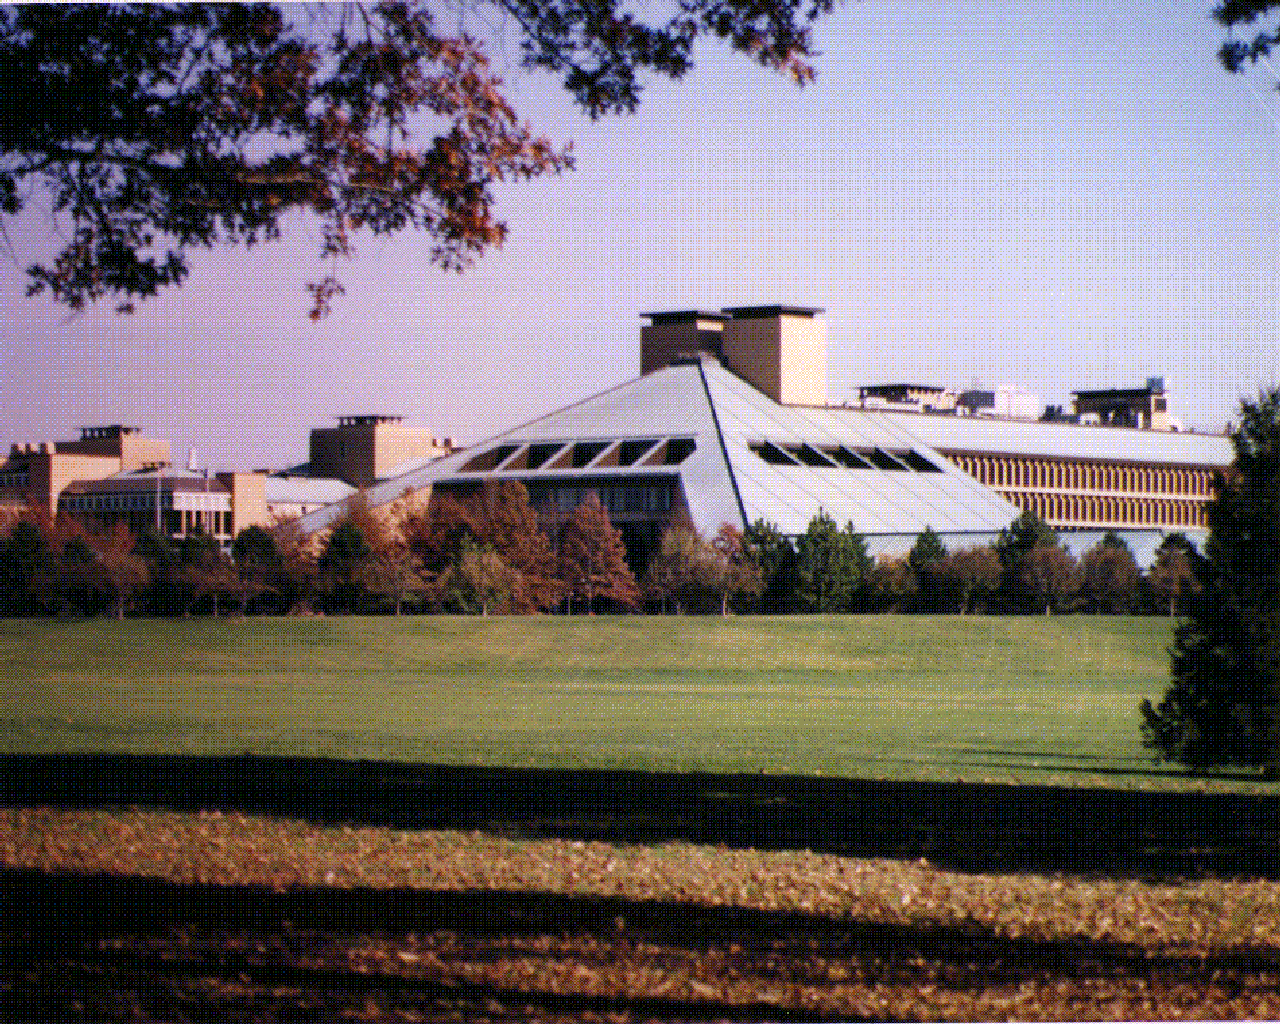
\includegraphics[width=0.6\textwidth]{assets/Lucent_HQ.png} 					\break
     		\break
     		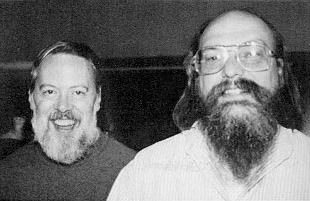
\includegraphics[width=0.6\textwidth]{assets/Ken_n_dennis.png}
     	\end{center}
		\end{column}
		
	\end{columns}
\end{frame}
%%---------------------------------------------------------------------

\subsection{Eksempler på brug af C}
\begin{frame}
	\begin{columns}
	
	\begin{column}{0.5\textwidth}
	\begin{itemize}
	\item{Kernen til dit Operativsystem er hovedsagligt skrevet i C}
	\item{C har inspireret mange sprog}
		\begin{itemize}
		\item{Java}
		\item{Swift}
		\item{Rust}
		\end{itemize}
	\item{Compilers og interpreters er ofte skrevet i C!}
	\item{C bruges i indlejret elektronik i stor stil!}
	\end{itemize}
	\end{column}
	
	\
	
	\end{columns}
\end{frame}

\end{document}

%%\begin{frame}[fragile]
	%%\begin{lstlisting}
		%%#include <stdio.h>

		%%int main(void)
		%%{
		%%printf("Hello world\n");
		%%return 0;
		%%}
	%%\end{lstlisting}
%%\end{frame}